\documentclass[main.tex]{subfiles}

\begin{document}
\sloppy
\chapter{Introduction}

The human brain has been a long standing topic of research in the scientific community. Many attempts have been made to model its behaviour using methods such as modeling the low level architecture on a neurological level \cite{frank1957perceptron} and a more abstract stochastic approach using  Bayesian inference \cite{bourlard1988auto} .

Being able to create a general form of artificial intelligence will allow for smarter robots that can learn and perform tasks in order to assist humans. However, robots are not easy to program and each task requires a specialised set of instructions for it to be executed properly. Such programs have various (dynamical) models and control policies embedded into them in order for the robot to function properly. Intrinsic system parameters, policies and controller gains are something which the human brain can learn over time \cite{friston2010free,knill2004bayesian, kawato1999internal}, yet a robot obviously has no such capability and tedious tweaking is required for everything to work properly.

There have been many attempts to reconcile the alluring anatomy of the brain and mathematical algorithms \cite{friston2003learning}, yet the most prevalent approach is generative modelling which has been widely adopted by the machine learning community. By combining the flexibility of \textit{neural networks} and probability theory these unsupervised learning algorithms can synthesise numbers, landscapes and even faces by learning latent features from training data and are called \textit{Deep Generative Models}. They are believed to hold the promise to general AI \cite{Goodfellow-et-al-2016}, yet  their application in robotics is scarce. Therefore, we are interested in applying such learning algorithms in the robotics field and more specifically in visuomotor control of an autonomous agent.

\section{Background}
In order to properly justify our research in this literature study we will define a problem space that needs solving. We will assume a 6-DOF robotic arm equipped with a camera as our autonomous agent. We wish for the agent to reach towards a visual point in space without having any knowledge of how the image is mapped to its internal kinematics. In other words, the agent has to figure out the positions of its joints based on image data which is also known as visual servoing. In addition, the agent should have some sort of \textit{generative model} which is a learned, low dimensional and stochastic representation of its kinematic model. In fact, the reason to have a low dimensional, or latent, representation is because storing all the possible states as high dimensional images makes computations difficult and impractical. 


Visual servoing has been explored extensively yet the implementations are generally model based \cite{hosoda1994versatile} or use reinforcement learning \cite{levine2016learning}. In other words, so far no application exists where a complex 6-DOF agent learns a generative kinematic model.


\section{Research Goal}

This practical example will be used for exploration and justification of various techniques. A set of requirements and conditions will be presented that can help us maintaining focus. However, in order to allow for further research and extension the research question will be formulated more generally.

In this literature study we aim to answer the following research question: 
\begin{quotation}
\begin{tabular}{|p{10cm}}
\textit{What unsupervised deep generative model allows an agent to infer latent system features by observing rich sensory data?}
\end{tabular}
\end{quotation}

Formulating this question in such a general way allows us to explore a wider range of literature, yet the requirements for the application keeps the research focussed. We have purposefully used the term \textit{latent system features} to indicate that the technique we propose should be valid for a wide range of applications such as both \textit{kinematics} and \textit{dynamics}. For simplicity we will not consider dynamics since robotic arms are well behaved in that respect [].

We define a set of requirements against which we can compare and contrast various techniques found in literature. Considering the learning nature of the brain using a generative model we also seek a technique that \textbf{i)} can infer a latent low dimensional representation from high dimensional sensory input such as images. Furthermore, the technique should allow us to \textbf{ii)} sample a generative model in order to make predictions. Such predictions could be used to estimate the velocity based on two images, for example.
Finally, since we are dealing with physical actuated systems the technique must also \textbf{iii)} provide tractable, robust and stable training dynamics.

In sections 2 and 3 we will discuss the background and relevance of neural networks and generative models, respectively. Section 4 investigates current state of the art techniques which have the potential of answering our research question. Section 5 compares and contrasts these methods against our set of requirements. We finally conclude with a short summary of this literature study and the chosen technique.

\chapter{Neural Networks}
Neural networks are the foundation of the machine learning field of research and have been studied for more than half a century. A wide variety of neural networks exists, each using a different architecture to perform specific tasks. We will focus on unsupervised learning which consists predominantly of optimisation problems (e.g. gradient descent).  

Recall that our agent is a robotic arm supplied with a camera. In terms of this literature study we aim to find a network (or a combination thereof) that can be used in vision based applications. In addition we want our agent to learn a low dimensional representation of its kinematics from the high dimensional visual data. Therefore, the network  must perform a form a dimensionality reduction. Since the landscape of neural networks is vast it is unpractical to give an overview of all possible types. Consequently, this chapter identifies only several neural networks and aims to justify why and how they are relevant to the research goal.

It is assumed that the reader has some working knowledge on neural networks. Therefore, the basic fundamentals of neural networks will not be covered in depth.

\section{Deep Neural Network}
A neural network is a set of connected nodes (neurons) which can have multiple inputs where each node then outputs a single value. Each connection has a weight and a bias. Each node takes the sum of the weights and biases connected to that node and is fed through some activation function. A clear graphical representation can be seen in figure \ref{fig:ann}

[figure of neural network]

Single layer neural networks, which only have one input layer and one output layer are only capable of modelling linear functions. In order to model non-linear functions, which is necessary in vision applications, we have to use \textit{deep} neural networks \cite{LeCun2015}. Such networks are characterised by having one or more \textit{hidden} layers in addition to the regular input and output layer.

What makes neural networks so powerful is their capacity to optimise their weights and biases through back-propagation. By optimising a cost function through, for example, a gradient descent method we can find the weights and biases that give us the most optimal results.

Deep neural networks with back propagation give us a very strong foundation which we can extend and apply to more exotic architectures.


\section{Autoencoder}
We have seen that deep neural nets form a solid foundation for various other types of networks. One of the goals of this literature study is to find a neural network that can learn a low dimensional (latent) representation from high dimensional data (e.g. images).

An autoencoder (AE) is used for such \textit{dimensionality reduction} applications. An AE network has a symmetric hourglass shape where the input and output layers have the same amount of nodes. The layers in between keep shrinking towards the center. The goal of the autoencoder is to ensure that the output is as similar as possible to the input. The hourglass shape forces an autoencoder to only extract relevant information which can be stored in a latent space (encoding) consisting of only several neurons as seen in figure \ref{fig:ae}. The latent representation is then fed through a decoder network which reconstructs the input. The network is penalised for errors in reconstruction. More formally, an AE learns a function $h$ with weights and biases, $w$ and $b$, that tries to approximate $x$ as much as possible, as shown in equation \eqref{eq:ae_approx}.

\begin{equation}
\label{eq:ae_approx}
  h_{w,b}(x) \approx \hat{x}
\end{equation}

% TODO: Add autoencoder figure

To summarise, autoencoders enable us to learn a low dimensional representation of our high dimensional data. Once an autoencoder is trained it can also be used to reconstruct corrupt images or interpret realistic scenes from simulated training data used in transfer learning \cite{zhuang2015supervised,kandaswamy2014improving}. This can be very beneficial when training our agent in a simulation, for example, and then using the trained network on a physical system.



\section{Boltzmann Machine}
[explanation is not entirely clear here, nor is the connection to the rest of this document]

Similar to an autoencoder, a Restricted Boltzman Machine (RBM) aims to reconstruct data in an unsupervised manner. As shown in figure \ref{fig:boltzmann_machine} an RBM has a single hidden layer and a layer which functions as both the input and output layer (i.e. visible units) which depends on the training phase. Interestingly, the RBM learns a \textit{stochastic} representation of the input data instead of storing variables in a latent space like the autoencoder does. This is exceedingly interesting since the we would have to deal with the variability of natural data as seen in images \cite{chen2003continuous}. 

During the forward pass of the training phase the activation value $a_j$ for a hidden node is determined by some probabilistic distribution $p(a_j|x_i;w_{ij})$ where $x_i$ is a visible node and $w_{ij}$ is the weight connecting node $i$ to node $j$. The type of this probability distribution is dependant on the implementation of the RBM. 

Now on the backward pass we let the RBM reconstruct the input and compare it to the real data, just as with an autoencoder. This comparison can be done with a Kullbackk-Leibler (KL) divergence where we try to minimise the difference in the two probability distributions, as shown in figure \ref{fig:kl_div}. We keep updating the weights until the optimisation converges or a maximum number of iterations (epochs) has been reached.

Thus, an RBM is a probabilistic spin on the AE where the RBM tries to \textit{infer} latent features of the dataset in order to make predictions when presented with new but comparable data. This is also called generative learning or \textit{generative modeling} which will be explored in more detail in the next chapter. Even though this neural network is similar to an AE, the stochastic nature of an RBM can be a preferred attribute since it resembles the variability of natural data.

\section{Convolutional Neural Network}
[Will obviously be expanded but it is trivial]

Images can have very large dimensions. A simple image that is only 20x20 pixels already requires 400 input neurons. Using a Convolutional Neural Network (CNN) allows us to take a relatively large image and use a scanning window to sample the image. This greatly reduces the complexity and dimensionality of the neural networks used.


\chapter{Generative Models}
In statistics and probability theory generative models are widely used to create a probabilistic representation of a target through observed variables. These generative models are capable of generating new data points from a joint probability distribution, unlike \textit{discriminative} models which have a conditional probability distribution.  Recall that the brain also uses inference and generative modelling to make predictions of the world which makes this method an interesting area of research.

Lately, generative models have gained a lot of traction in the machine learning community due to their ability to infer features from a probabilistic dataset where not all variables can be observed \cite{Goodfellow-et-al-2016}. An agent which has the capability to infer latent features of the world or itself and make predictions by sampling a generative model could lead to more interesting behaviour in terms of autonomous systems. For example, our agent could use such a generative model to learn admissible kinematic states based on training data in the form of images.

In this chapter we will discuss the general math behind generative models, some examples on how they are being used in the machine learning community and why it is relevant in this literature study.

\section{Joint Probability Distribution}
Take $z$ to be a random \textit{unobserved} variable and $x$ to be a random \textit{observed} variable.
A generative model is capable of generating new values for combinations of $x$ and $z$ and is given by
\begin{align}
    \label{eq:generative_model}
    p(x,z) = p(x|z)p(z).
\end{align}

In words, given a prior distribution, $p(z)$ and the likelihood, $p(x|z)$ we can generate new data for combinations of $x$ and $z$. However, the question remains how we obtain $p(x|z)$, the distribution which gives us observable variables based on the hidden variables. This might seem non-intuitive since we wish to learn the latent features from observations. This is true, but in order to make \textit{predictions} on the observed variables (posterior) we need to find this likelihood $p(x|z)$ as seen in Bayes' rule
\begin{equation}
  \label{eq:bayes_rule}
  \underbrace{p(x|z)}_{\text{likelihood}} = \dfrac{\underbrace{p(z|x)}_{\text{posterior}} \underbrace{p(x)}_\text{evidence}}{\underbrace{p(z)}_\text{prior}}.
\end{equation}

In terms of machine learning we see from equation \eqref{eq:bayes_rule} that expressions where the hidden variable $z$ is given are obtained through training. On the other hand, expression with $x$ given use inference to obtain $z$.

Going back to the predictive nature of the brain, we are interested in knowing the true (unobservable) state of the world based on observed variables. Essentially, we are interested in the posterior distribution $p(z|x)$. With this we can \textit{infer} a model of the world from which we can then sample to make predictions. This is what Bayesian inference is used for.

\section{Bayesian Inference}
When dealing with a dynamical system of which one or more states can not be directly measured one could apply Bayesian inference in order to infer that hidden state based on a model. A well known example is the Kalman Filter \cite{bishop2001introduction}. We are interested in the underlaying technique of the Kalman Filter, namely Bayesian inference in order to infer hidden variables from high dimensional data. Practically speaking, for our agent we would like to infer the kinematical model based on images.

From the previous section we have seen how we can use a generative model in order to produce new values for $x$ and $z$. However, this generative model first has to be trained in order for it to produce anything meaningful. For example, a trained generative model could be able to predict the position of a 3-DOF robotic arm from two \textit{unseen} consecutive visual representations \cite{watter2015embed}.

A generative model is able to do so by sampling the posterior probability distribution which is dependent on the marginal likelihood as shown in \eqref{eq:inference-integral}.
\begin{align}
    \label{eq:inference-integral}
    p(x) = \int p(x|z)p(z)dz
\end{align}

Even though the integral in equation \eqref{eq:inference-integral} can be solved theoretically, it is far from practical when dealing with the amount of data generally used in machine learning. In other words, evaluating the marginal likelihood (or evidence) in \eqref{eq:inference-integral} is intractable leading \eqref{eq:bayes_rule} by substitution to also become intractable.

Happily, recent advances in machine learning produced solutions which can approximate the intractable true posterior $p(z|x)$ making inference possible.

\section{Variational Inference}

As we have seen Bayesian inference is a powerful tool to use statistics in order to find the probability of an outcome based on a generative model. However, the integral over the likelihood as shown in equation \eqref{eq:inference-integral} is intractable causing the true posterior, $p(z|x)$ to also be intractable. In order to infer the kinematics of our robotic agent and be able to generate new configurations we need to be able to build the generative model and approximate the posterior. Variational inference gives us the tools for that. 

Let $p(z|x)$ be a probability distribution which we can not fully observe, only sample. In order to find $p(z)$ we need to sample for all combinations of $x$ and $z$ which is intractable, as we have seen. There are sampling methods such as Markov chain Monte Carlo (MCMC), yielding exact samples from the target distribution, but these are very computationally heavy and are best suited for smaller datasets \cite{blei2017variational}. Variational inference (VI) is a method that approximates the probability density and therefore does not guarantee the same accuracy as MCMC. However, the nature of VI allows for very fast and efficient optimisation techniques such as gradient search. Assuming the geometry of the distribution to be approximated is moderately complex and well behaved, the inaccuracy of VI is acceptable and its speed then outweighs the benefits of other slower methods such as MCMC.

In order to solve the intractability of \eqref{eq:inference-integral} and \eqref{eq:bayes_rule} we can introduce a recognition model $q(z|x)$. The recognition model is an approximation of the true distribution $p(z|x)$. Let the recognition model and posterior distribution be parameterised by $\phi$ and $\theta$, respectively. For example, if the posterior is a normal distribution $\mathcal{N}(\mu,\sigma^2)$ parameterised by $\theta$ then the set is given by $\theta = \{\mu, \sigma\}$. This will lead to the following notation $q_\phi ( \cdot)$ for the approximation and $p_\theta (\cdot)$ for the true distribution.

The posterior distribution is approximated by varying the parameter $\phi$ such that the KL-divergence between $q_\phi(\cdot)$ and $p_\theta(\cdot)$ are minimised up to an added constant called the lower bound (ELBO or $\mathcal{L}$). Formally we solve the optimisation problem given by

\begin{equation}
\label{eq:elbo}
  \log p(x) = \argmin_{q_{\phi}(z)} D_{KL}\infdiv{q_\phi(z)}{p_\theta(z|x)} + \mathcal{L}(\phi,\theta)
\end{equation}

where $\mathcal{L} \leq \log p_\theta(x)$ since the KL-divergence is always $ \geq 0$. This shows that this optimisation will always be an approximation since \eqref{eq:elbo} will always have an added constant in the form of the lower bound $\mathcal{L}$. Finding the right parameters now becomes gradient search problem which can be handled by neural networks for fast convergence and parallel computing \cite{rezende2014stochastic,kingma2013auto}. 

\chapter{Techniques}
So far we have investigated the fundamentals of neural networks, their implementations and statistics theory in terms of generative models. We have seen that generative models give us the ability to model the variance of natural data such as images. We can use such models to then make predictions. This is exceedingly interesting in robotics where we could use state of the art machine learning (ML) techniques in the control of robots. Returning to our goal, we want our agent to be able to infer its kinematics from images during training and then perform some action when a prior is given.

In literature two very prominent techniques are apparent that can potentially help us with our desired goal. Variational Autoencoders and Generative Adversarial Networks are both neural network based generative models \cite{kingma2013auto,goodfellow2014generative}. These techniques are researched heavily in the machine learning community where they can perform a wide array of tasks such as image synthesis, action forecasting from static images \cite{walker2016uncertain} and latent dynamic embedding for control \cite{watter2015embed}. This chapter will give an overview of the workings of both techniques. Since MNIST \footnote{MNIST is a database containing images of handwritten digits from 0-9 and is widely used as a benchmarking dataset for machine learning. \url{http://yann.lecun.com/exdb/mnist/}} is a go-to benchmarking dataset for ML algorithms we will also identify the performance of the VAE and GAN based on this dataset. For each technique we will discuss their workings after which we identify publications that are relevant to our research for our autonomous agent.
 
\section{Variational Autoencoder}
In the previous sections we have discussed the neural network architecture for an autoencoder and variational inference in generative modelling. One of the problems in Bayesian inference is the intractability of the posterior. A variety of algorithms exist which approximate that probability density by means of variational inference. However, these methods are relatively slow or require an analytical solution of the expectations. An efficient method is proposed by \cite{kingma2013auto} which is the Variational Autoencoder (VAE), a generative modelling neural network. Its power lays in the ability to jointly learn the parametrisation of the posterior distribution $q_\phi(z|x)$ and the likelihood $p_\theta(x|z)$.

\subsection{Background}
Similarly to a regular autoencoder, the VAE tries to reconstruct the input but it does so by minimising two loss functions: the latent loss given by the same equation as seen in equation \eqref{eq:elbo}, and the generation loss which is a simple mean square error given by
\begin{equation}
  \lVert x-\hat{x} \rVert^2
\end{equation}
where $x$ is the real data and $\hat{x}$ is the generated data. 

[insert relevance to RBM]

\begin{figure}[bt]
    \centering
    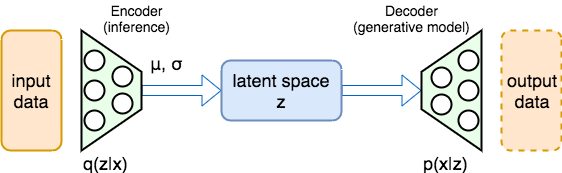
\includegraphics[width=0.95\textwidth]{VAE2}
    \caption{A Variational Autoencoder ingests data into an encoder network which learns $\mu$ and $\sigma$ to parameterise the recognition model $q_\phi(z|x)$. The decoder then samples from the latent space which is constrained to be $\mathcal{N}(0,1)$ and tries to reconstruct the input by minimising the KL-divergence between $q$ and $p$.}
    \label{fig:vae}
\end{figure}

Recall from the previous chapter that in variational inference we try to optimise the parameters for the recognition density $q_\phi(z|x)$ and the likelihood $p_\theta(x|z)$. The VAE consists out of two neural networks, an encoding network and a decoding network, as seen in figure \ref{fig:vae}. When a VAE is used for inferencing latent variables from images often convolutional networks are used to reduce the network size. In short, a VAE learns the following two things: the parameters for the recognition model $\phi$ and the parameters for the likelihood $\theta$ which are used to sample the latent space $z$.

The encoder network of the VAE represents the posterior approximation $q_\phi(z|x)$. The input of the network is a dataset from which we want to learn the latent features and the output is the set of parameters $\phi = \{\mu,\sigma\}$ assuming a Gaussian distribution in the dataset. More formally, the encoder network represents a probability distribution given by
\begin{equation}
  \label{eq:recognition_model}
  q_\phi(z|x) = \mathcal{N}(z|\mu(x), \sigma(x)^2)
\end{equation}
 
where the parameters $\mu$ and $\sigma$ can be seen as arbitrary mapping functions learned by the neural network. The objective of the encoder neural network is to minimise the KL-divergence between the learned latent space and the unit Gaussian as shown below.
\begin{equation}
  \argmin D_{KL}\infdiv{\mathcal{N}(z|\mu(x), \sigma(x)^2)}{\mathcal{N}(0,1)}
\end{equation}

This constraint forces the VAE to learn sufficiently varied latent variables and not just how to memorise the dataset.

On the right hand side of figure \ref{fig:vae} we have the decoder network that represents the likelihood $p_\theta(x|z)$. Since we let the decoder samples from the simple latent space $z \sim \mathcal{N}(0,1)$, the complexity of the dataset is instead captured by the neural network $p_\theta(x|z)$\cite{zhao2017towards}. Both $\theta$ and $\phi$ are learned by back-propagating the error from the latent and generation loss through the neural network. Recall the generative model is given by \eqref{eq:generative_model}, thus by sampling the likelihood and the latent space we can reconstruct the image.

As many other ML techniques, the VAE is benchmarked using the MNIST dataset. Given an MNIST dataset the VAE can learn the latent features of the numbers from which it can then \textit{generate} a new but similar dataset. When the latent space $z$ is projected in 2D space (which is used for demonstrating latent feature learning) we can see how the VAE interprets the numbers and how the latent features are linearly interpolated.

[MNIST figure]

\subsection{Applications}
Variational autoencoders have seen a widespread adoption in the machine learning community for learning latent features in high dimensional data. Aside from \textit{dreaming} of landscapes and handwritten digits there are many applications which demonstrate the use of VAEs and how it can be used in our research.

Recall that our agent is a robotic arm with 6 degrees of freedom and has a camera. Our goal is for that robot to learn its own internal kinematics in the form of a generative model. This would mean that once we present the agent with a prior belief (a position in space in the form of an image) we should be able to generate a trajectory towards that point \textit{without} performing direct inverse kinematics. The VAE could be a very useful tool to achieve our goal. Therefore, we will explore some examples in literature. 

In a recent publication a VAE is trained with thousands of videos after which it is able to predict the trajectory of a set of pixels in a static image \cite{walker2016uncertain}. As is usual in vision applications, a convolutional neural network was used to reduce the computation time and dimensionality of the network. Considering our research, a trained VAE that can predict the next state of a robotic arm from an image can be interesting. 

Another important publication shows how a Kalman filter can be learned using multiple techniques including a VAE \cite{krishnan2015deep}. The authors propose the Deep Kalman Filter (DKF) which extends the inference network with an action variable $u$ such that recognition model becomes $q_\phi(\vec{z} \mid \vec{x}, \vec{u})$ where the arrow indicates a sequence. The neural network is parametrised by $\theta = {\alpha, \beta, \kappa}$ which allow the authors to learn the mapping functions for the latent space and observation space.
\begin{equation}
  \label{eq:deep_kalman}
  \begin{split}
  z_t &\sim \mathcal{N}\left(G_\alpha (z_{t-1}, u_{t-1},\Delta_t), S_\beta(z_{t-1}, u_{t-1},\Delta_t) \right) \\
  x_t &\sim \Pi\left(F_\kappa(z_t)\right)
  \end{split}
\end{equation}

The generative model for the Kalman filter is given by equation \eqref{eq:deep_kalman} where the latent space is normally distributed by the given non linear mapping functions, $G_\alpha$ and $S_\beta$, which are dependent on the previous latent state, action and time difference. By restricting the functional forms of the mapping functions, different Kalman filters can be trained demonstrating the flexibility of this framework. This method are a derivative thereof can be extremely beneficial for our autonomous agent when control actions have to be predicted. However, this is under the assumption that the DKF is trained with both sensory observations \textit{and} corresponding actions.

Finally, another promising example is a publication that has made an effort to learn the latent dynamics of various systems on which stochastic optimal control \cite{watter2015embed} could be performed. Their method Embed to Control (E2C) uses multiple VAEs and an iterative linear quadratic regulator (iLQR) in order to learn the swing up of an inverted pendulum. In short, they accomplish this by stacking two images of a simulated pendulum which represent their states at $s_t$ and $s_{t+1}$ and training the VAE with a large dataset of such stacks. The VAE is then able to learn the state space representation of the pendulum which the iLQR controller can then use, given a desired state, to learn a swing up. 

The E2C method is a promising algorithm which has the potential to be extended to larger degrees of freedom, allowing for control of complex robotic systems using raw sensory information. As long as the latent space has the Markov property, stochastic optimal control can be applied to a latentx kinematic model which has been learned in an unsupervised manner \cite{matsubara2014latent}. 

\section{Generative Adversarial Networks}
[Mention that GANs can not model discrete data]

Another well known deep generative model is the generative adversarial network (GAN). It is a technique based on a zero-sum game where two neural networks are competing against each other \cite{goodfellow2014generative}. Similarly to a VAE, a GAN learns a generative model from training data as well. However, a GAN does not require an inferencing network.

\subsection{Background}

Recall from chapter 3 that the generative model is given by equation \eqref{eq:generative_model} for which we need multiple dependent equations leading to intractable calculations. Where the VAE circumvents that by using a recognition model to approximate the posterior, the GAN completely cuts out the inference step. It does so by simultaneously training two neural networks, the generator ($G$) and the discriminator ($D$), which play a minimax game as shown in figure \ref{fig:gan_minmax}. The aim of the game is for the generator to create sufficiently believable samples that the discriminator can no longer discern what is real and what is generated. 

\begin{figure}[h]
    \centering
    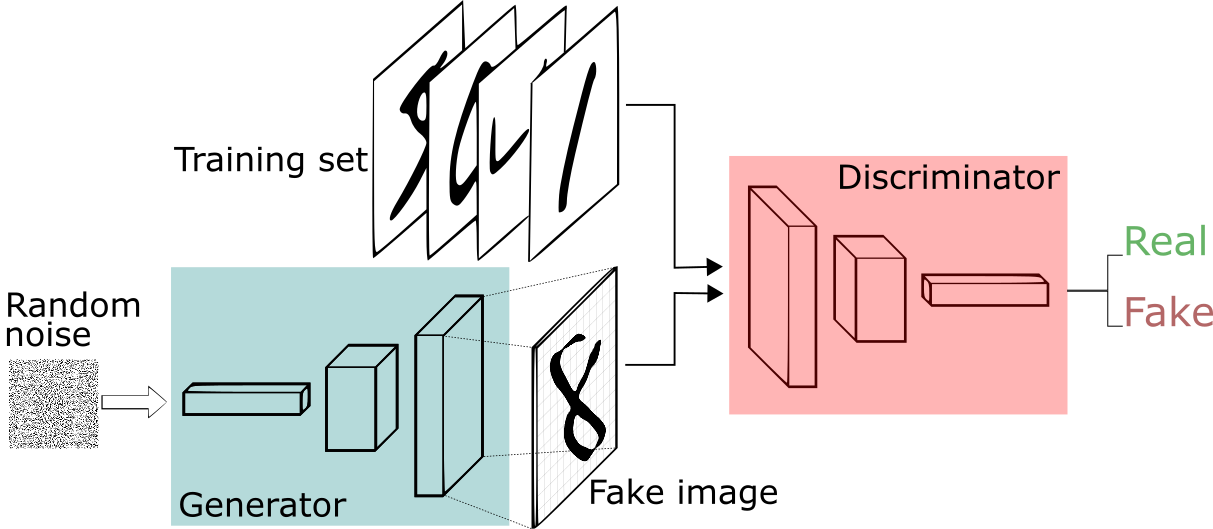
\includegraphics[width=0.95\textwidth]{gan_minmax}
    \caption{A generative adversarial net samples from a simple gaussian distribution. Both the generator and discriminator neural nets are optimized. The Jensen-Shannon divergence is used to calculate the loss between the distributions which is then back-propagated through the networks. needs citation: https://sthalles.github.io/intro-to-gans/}
    \label{fig:gan_minmax}
\end{figure}

The generator network of a GAN is fairly simple. The GAN does not make any approximations to the posterior, unlike the VAE, instead it simply assumes the latent space distribution $p(z)$ to be random noise given by $\mathcal{N}(0,\mathbf{I})$ where $\mathbf{I}$ is the identity matrix. The dimensionality of the identity matrix and thus that of the latent space is heuristically determined.

The generator network represents a mapping to the data space as $G_\theta(z)$ where $\phi$ are the parameters of the neural network. Statistically, the generator would represent the likelihood $p(x|z)$ which combined with the prior $p(z)$ is the generative model as we've seen in equation \eqref{eq:generative_model}.

The discriminator network $D_\gamma(x)$, parameterised by $\gamma$, is a lot simpler. It outputs a probability scalar indicating whether its input $x$ came from the real data or the generative model $G_\theta(z)$. In words, the generator constantly tries to improve itself to "fool" the discriminator network. On the other hand, the discriminator network constantly tries to become better at catching the generator network. Both networks are jointly trained with the following value function $V(G,D)$:
\begin{equation}
\label{eq:gan_minimax}
  \min_{G} \max_{D} V(D,G) = \mathbb{E}_{x\sim p_{data}(x)} [\log D(x)] + \mathbb{E}_{z\sim p_z(z)}[\log(1-D(G(z)))].
\end{equation}

As with most ML techniques the GAN is also benchmarked on the MNIST dataset. We see in figure \ref{fig:gan_mnist} that the GAN performs really well in generating new handwritten digits. Also, linearly interpolating between the coordinates in $z$-space shows that the algorithm has clearly learned latent features as shown in figure \ref{fig:gan_mnist_interp} .

\begin{figure}[htb]
    \centering
    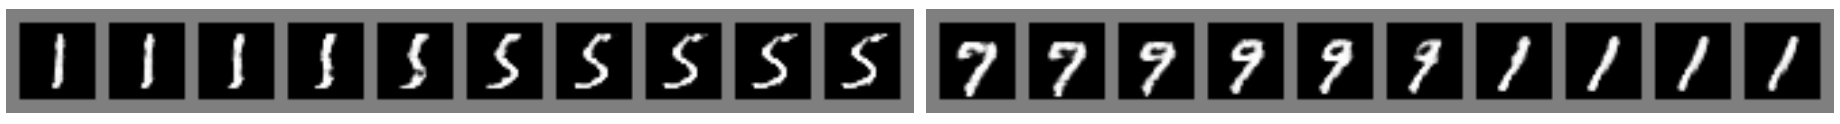
\includegraphics[width=0.95\textwidth]{gan_interp}
    \caption{Digits obtained by interpolating between latent variables.}
    \label{fig:gan_mnist_interp}
\end{figure}


\subsection{Applications}
As with many other ML techniques, the GAN too was originally benchmarked by synthesising images. Fortunately, it has seen immense adoption and widespread use in the scientific community, probably more so than the VAE. Some examples will be discusses in this section demonstrating the power of GANs.

[will be expanded with literature i'm still trying to understand]

Finally we discuss an interesting publication on using GANs for learning forward and inverse models for motor control of a 2-DOF simulated robotic arm \cite{lenninger2017generative}. The model is trained by feeding it simulated current $S_t$ and future $S_{t+1}$ states caused by an input $u_t$. The states of the links are defined as vectors are given by $S_{t} = \{X_t(\theta_t),\theta_t, \dot{\theta}_t\}$, where $X_t(\theta_t$) is the position of the end-effector. The future state $S_{t+1}$ is calculated by the simulator. During training the generator tries to reconstruct the future state and the discriminator compares it to ground truth from the simulator. Ultimately, both the forward model and the inverse model of the arm are learned under the generative model. This allows the arm to either find the control input that has caused a change in state or find the next state given a control input.

\chapter{Conclusion}
Our goal is to find an unsupervised technique which can learn latent system features to be used in robotic applications, more specifically in applications requiring vision. In this literature study we have investigated  two important machine learning techniques, namely, variational autoencoders (VAE) and generative adversarial networks (GAN). These deep generative models are actively researched in the ML community and are believed to hold the promise for true AI. Combining such a state of the art learning algorithm in the field of robotics could pave the way to fully autonomous systems. In terms of our proposed robotic agent, we seek a technique which allows it to learn its internal kinematics in an unsupervised manner after which it can perform a task given a prior belief in the form of an image.

In this literature study we have found that the variational autoencoder is the most suitable method to proceed with our research purposes. This is according to the three main criteria which have been defined in the introduction and will be discusses next.

Firstly, VAEs are explicitly designed to learn latent features from high dimensional data. Our aim is to observe raw sensory information (e.g. images) and learn a reduced representation. This \textit{inferencing} step allows us to extract meaningful information from a scene after which we can make predictions. In contrast to VAEs, GANs have no support for this requirement unless modified \cite{mescheder2017adversarial,chen2016infogan}. For example, if we wish to supply our agent with a prior belief, for a VAE we could represent that as a simple image of which the latent features can be inferred. For a GAN this becomes somewhat complicated as the prior belief has to be directly embedded into the latent space since there is no inference step. 

Secondly, both VAE and GAN learn a generative model from which we can sample in order to make predictions based on a prior belief. In this case both techniques are equal as they both have a generative model which can be sampled and are flexible in terms of scalability. However, it is important to note that VAEs require differentiation through the hidden units due to the nature of the training algorithm \cite{goodfellow2014generative}. Thus VAEs can not have discrete latent variables. How this will affect the discrete nature of digital sensors such as encoders is unknown.

Thirdly, VAEs have a robust training algorithm and good convergence. Even though both VAEs and GANs have their advantages and disadvantages, their training dynamics are very different which are crucial in our robotic application. In literature we see that VAEs take longer to train than GANs. Where the GAN has $O(n)$ time-complexity the VAE requires $O(n \log n)$ for training to complete []. In addition we see that  in contrast to GANs, VAEs produce blurry images in many benchmarks such as CIFAR-10. It is still unknown what causes the blurriness. In terms of robotic application we do not know how this effect will be translated but it is imaginable that a VAE will have a larger variance between possible states as opposed to a GAN. However, this performance does not outweigh the training dynamics where the GAN falls short. Namely, GANs are notoriously hard to train \cite{Goodfellow-et-al-2016, arjovsky2017towards}. Because the GAN tries find the Nash-equilibrium, the convergence of the gradient descent can fail under high dimensional parameters \cite{goodfellow2014distinguishability}. It is possible to alleviate some of the issues with the GAN by using a modified training algorithm \cite{arjovsky2017wasserstein}. Thus, stability and convergence of a VAE during training outweigh the high performance of a GAN. In the case that the performance for sharper images is deemed necessary, there are various options available \cite{mescheder2017adversarial, rezende2015variational, salimans2015markov}.

Finally, for future work we recommend further investigation of variations of the proposed methods. Machine learning is very much an active field of research and it is quite commonplace for techniques to be combined such as VAEs with GANs \cite{mescheder2017adversarial,hu2017unifying}. In case the performance of the \textit{vanilla} methods seem to underperform, such combinations can be investigated to improve results. In addition, generative models tend to not have an interpretable visual representation \cite{feichtenhofer2018have}. Therefore, further investigation can be beneficial in order to better understand what such a model has learned.

In summary, variational autoencoders offer a flexible and novel way for an autonomous agent to learn latent features of its own internal system or its surroundings. If this method is coupled with an implementation for \textit{active} exploration of the environment, this research could lead to a novel approach for creating real autonomous agents which can learn to understand the world they live in.

\newpage
\renewcommand\bibname{References}
\bibliographystyle{unsrt}
\bibliography{references}

\end{document}
